\section{Experiments}
\label{sec:exp}

We complement the theory with exact computational experiments addressing four questions: (a) how much profit reallocation improves over the baseline on trees; (b) whether the gains survive dropping \cref{asp:homo,asp:posi}; (c) how they scale with the tree depth $d$ and branching factor $m$ in regular trees; and (d) whether they persist on an irregular tree.

\subsection{Setup}

We consider two families of tree structures. The first is \emph{complete $m$-ary trees} of depth $d$: the root originates the data and every non-leaf player has $m$ children, giving levels $0,\ldots,d$. By the level-symmetry of the tree under a Markovian valuation process, all players on the same level share the same equilibrium strategy, so it suffices to compute $d+1$ representative strategies. The second is the \emph{irregular} tree of \cref{fig:tree-notation}: a $7$-player instance with root $r$ and children $u,l$, where $l$ is a leaf, $u$ has children $uu$ (a leaf) and $ul$, and $ul$ has two leaf children $ulu,ull$---so branching and depth vary across nodes (depths range from $1$ to $3$). Lacking level-symmetry, it is solved without any symmetry reduction. All equilibria are computed exactly with \cref{alg:exact}.

\paragraph{Valuation models.}
Each child's valuation follows a local random walk on the grid: from a parent $i$ with value $v_i = w_k$, each child $j$ generates $k'$ independently in one of $k-2,\dots,k+2$ with equal probability (clipped into $[0,2d]$ for M2) and set $v_j = w_{k'}$. The four models share this transition and differ only in the values of $\{w_k\}$s. Specifically:
\begin{itemize}[left=0em]\itemsep0.1em
\item \textbf{M1} (homogeneous, positive): $w_k = e^{(k-2d)/2}$, $k=0,\ldots,4d$, root $v_r = w_{2d} = 1$; satisfies both \cref{asp:homo,asp:posi}.
\item \textbf{M2} (non-homogeneous, positive): $w_k = k/2d$, $k=0,\ldots,2d$, root $v_r = w_0 = 0$; violates homogeneity.
\item \textbf{M3} (homogeneous, non-positive): $w_k = (-1)^k e^{(k-2d)/2}$, $k=0,\ldots,4d$, root $v_r = w_{2d} = 1$; violates positivity.
\item \textbf{M4} (non-homogeneous, non-positive): $w_k = (k-2d)/2d$, $k=0,\ldots,4d$, root $v_r = w_{2d} = 0$; violates both.
\end{itemize}
% Only M1 is covered by our theory, while M2--M4 test robustness.

\paragraph{Mechanisms.}
We compare four budget-balanced PRMs. For a trade $m$ with ancestors $\Path(m)$, writing $\ell_m \coloneqq |\Path(m)|$ and, for $k \in \Path(m)$, $s(m,k) \coloneqq \mathrm{depth}(\Parent(m)) - \mathrm{depth}(k) \in \{0,\ldots,\ell_m-1\}$ for the number of steps from the direct seller $\Parent(m)$ up to $k$:
\begin{itemize}[left=0em]\itemsep0.1em
\item \textbf{RAW} (baseline, \cref{def:baseline}): the direct seller keeps everything, $\pi(m,\Parent(m)) = 1$ and $\pi(m,k) = 0$ for $k \neq \Parent(m)$.
\item \textbf{TBDS}: a fixed-ratio rule with $\alpha = 0.5$ that shares a trade's payment geometrically up the ancestors---$\pi(m,k) = (1-\alpha)\,\alpha^{\,s(m,k)}$ for $k \neq r$, with the root absorbing the remainder $\pi(m,r) = \alpha^{\,\ell_m-1}$; this mechanism is originally proposed by \citet{xin2025tbds} and is a special case of our PRMs.
\item \textbf{AVE}: each trade's payment is split uniformly among its ancestors, $\pi(m,k) = 1/\ell_m$ for every $k \in \Path(m)$.
\item \textbf{OPT}: a budget-balanced PRM optimized by a zeroth-order optimizer maximizing equilibrium welfare, run separately for each model.
\end{itemize}

Note that RAW, TBDS, and AVE are model-independent PRMs, while OPT relies on the underlying distribution $\calF$.


\paragraph{Metrics.}
We report two equilibrium quantities: \emph{social welfare} $\SW=\sum_{i\in\calI}u_i(\tbmp^*,\tbmx^*)$ and \emph{transaction volume} $\mathrm{TV}=\sum_{i\in\calI\setminus\{r\}}\Pr[y_i=1]$, the expected number of completed trades. Both are evaluated \emph{exactly} by the forward dynamic program, so every reported value is exact.

\subsection{Results}

\begin{table}[t]
\centering
\small
\caption{Equilibrium transaction volume (TV) and social welfare (SW) at $(d{=}5,\,m{=}2)$, computed exactly. RAW is the baseline; TBDS~\citep{xin2025tbds} the fixed-ratio rule ($\alpha{=}0.5$); AVE and OPT are instances of our budget-feasible family.}
\label{tab:exp}
\begin{tabular*}{\textwidth}{@{\extracolsep{\fill}} l cccc cccc @{}}
\toprule
& \multicolumn{4}{c}{Transaction Volume} & \multicolumn{4}{c}{Social Welfare} \\
\cmidrule(lr){2-5}\cmidrule(lr){6-9}
Mechanism & M1 & M2 & M3 & M4 & M1 & M2 & M3 & M4 \\
\midrule
RAW  & $2.69$  & $21.17$ & $0.66$  & $5.74$  & $36.70$  & $5.56$ & $7.47$  & $2.37$ \\
TBDS & $8.10$  & $26.03$ & $3.68$  & $9.94$  & $75.99$  & $6.76$ & $14.03$ & $3.61$ \\
AVE  & $12.83$ & $37.27$ & $4.48$  & $12.91$ & $92.81$  & $8.23$ & $19.72$ & $4.33$ \\
OPT  & $42.80$ & $46.33$ & $16.81$ & $20.15$ & $140.00$ & $9.33$ & $39.14$ & $5.34$ \\
\bottomrule
\end{tabular*}
\end{table}


\paragraph{Welfare and trade improvements (a, b).}
\cref{tab:exp} reports both metrics for a representative configuration ($d=5$, $m=2$). Every PRM improves over RAW across all four models, including those violating \cref{asp:homo,asp:posi}. Averaged over the four models, the model-independent AVE and TBDS already yield large gains over RAW---$289\%/112\%$ and $189\%/67\%$ in transaction volume/social welfare.
The results suggest that PRMs remain effective across diverse scenarios, even when \cref{asp:homo,asp:posi} no longer hold.
%  As AVE and TBDS are fixed closed-form rules needing no per-market tuning, we regard them as the deployable mechanisms and OPT as the welfare ceiling of the design space.

% These margins are large because the baseline market nearly collapses on deep, branching trees---upstream sellers capture none of the downstream value and price most buyers out---whereas reallocation revives trade throughout.

\begin{figure}[t]
\centering
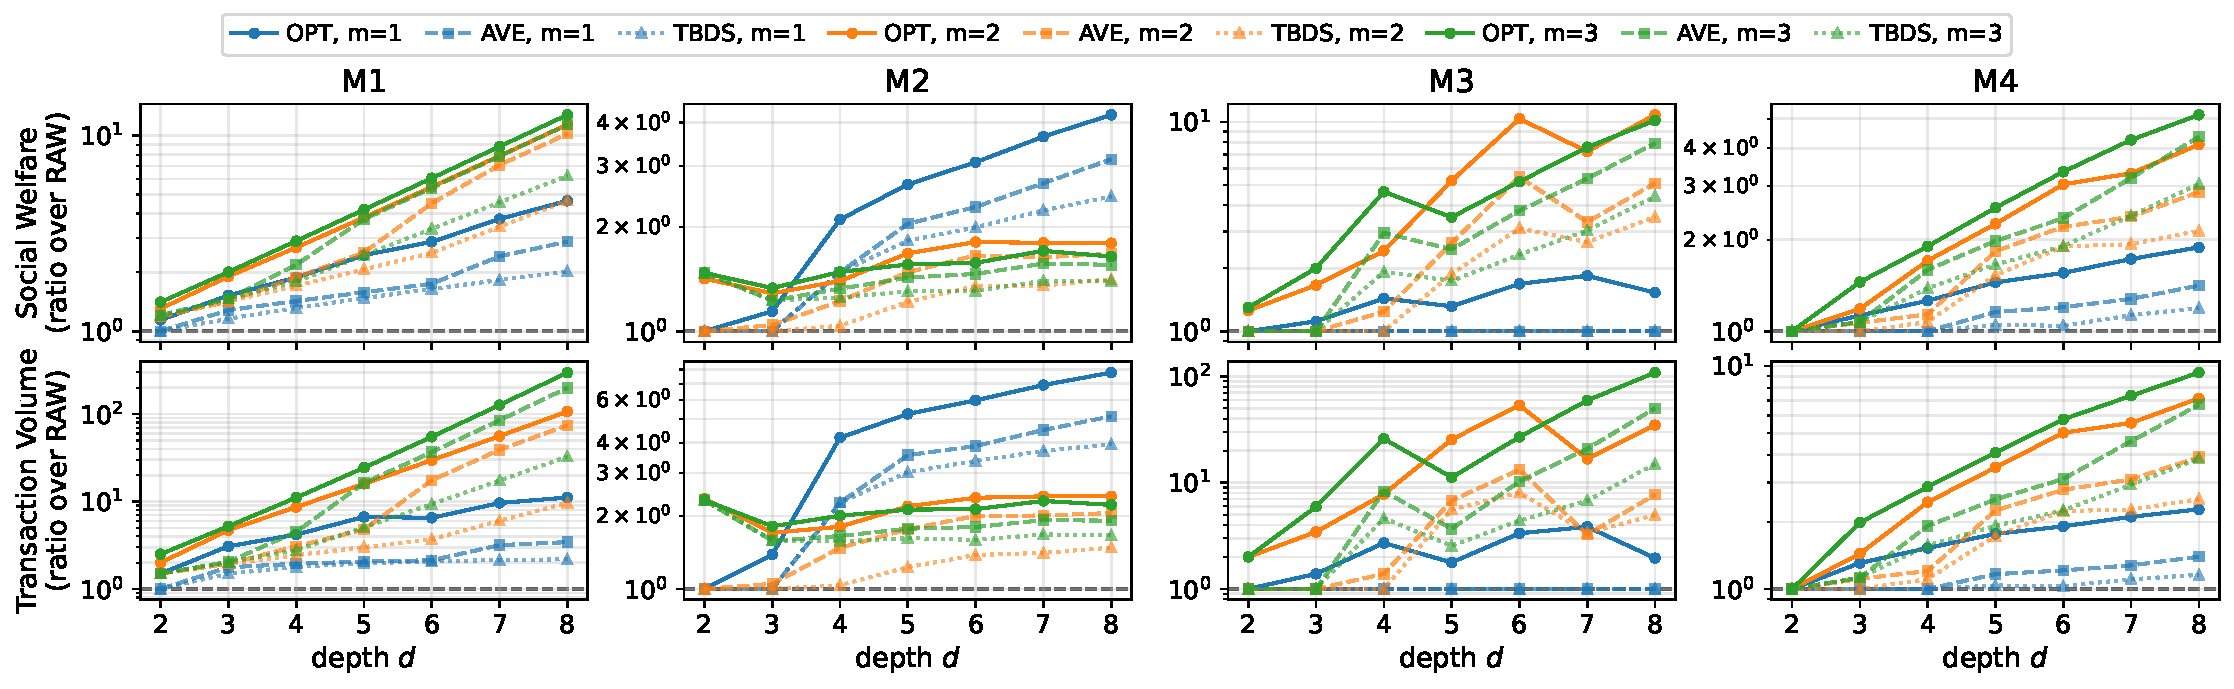
\includegraphics[width=\textwidth]{Materials/exp_vary.pdf}
\caption{Equilibrium social welfare (top) and transaction volume (bottom) of the AVE and OPT mechanisms, expressed as a ratio over the baseline RAW mechanism, as the tree depth $d$ varies from $2$ to $8$. Each column is one valuation model; colors denote the branching factor $m \in \{1,2,3\}$ ($m=1$ is the chain). Ratios above the dotted line ($=1$) indicate that profit reallocation improves upon the baseline. The advantage generally grows with depth and branching.}
\label{fig:exp-vary}
\end{figure}


\paragraph{Scaling with depth and branching (c).}
Varying $2 \le d\le 8$ and $m\in\{1,2,3\}$ with results shown in \cref{fig:exp-vary}, the advantage of PRMs over RAW generally grows with both depth $d$ and branching $m$---deeper, bushier trees create more downstream profits to reallocate---and is robust to violations of positivity and homogeneity.

\paragraph{Irregular trees (d).}
We report the results of the \emph{irregular} tree structure as in \cref{fig:tree-notation}, shown in \cref{tab:exp-irregular}, \cref{sec:app-experiments}. The picture is unchanged---PRMs beat RAW for every model, indicating that the benefit of PRMs is not specific to symmetric trees.
